\subsection{缓存教师中心误差与末期噪声}

记 $h=U-f$、$R=C_qh$、$D=R/\eta$、$\psi=\nabla\log p$、$\varphi=\psi-\E_q\psi$。真实 BPO 梯度为 $\bm G=\E_qD\psi=\E_qD\varphi$。若缓存 $\widehat K=K+e$，使用未修正的 score 更新会产生偏差 $-e\E_q\psi$。改用中心化 score 后，任意固定 $e$ 都不改变梯度期望，却保留随机性。尤其在 $p=m$，$D=0$，
\begin{equation}
 g=-e\varphi,\qquad
 \Var_q(g)=e^2\E_q\|\varphi\|^2.
\end{equation}
若中心用 $M$ 个独立样本估计、方差为 $\sigma_K^2/M$，再对中心误差求平均，就得到 $\sigma_K^2\E_q\|\varphi\|^2/M$ 的末期噪声。完整条件求和时，$\E_q\varphi=0$ 会精确消掉这一项；因此完整词表 BPO 不需要通过教师中心估计器控制这一采样噪声来源。

可以利用学生反馈估计中心：令 $y=C_qU/\eta-A$，则 $\E_qy=K$，而
\begin{equation}
 \Var_qy=\Var_qD=\frac{2\mathcal L_{\mathrm{BPO}}}{\eta}.
\end{equation}
独立辅助 action 上的 $y$ 估计在拟合到 target 时方差消失，优于仅依靠 teacher 监督的固定中心噪声底；它通常没有逐样本统一范围。下面将这个差分进一步对称化，同时消去学生条件中心。
\subsection{不显式估计两个中心的 BPO 二样本损失}

令 $a,b\overset{\mathrm{iid}}\sim q$，定义
\begin{equation}
 \widehat\ell_2=\frac{[h(a)-h(b)]^2}{4\eta},\qquad
 \widehat{\bm G}_2=\frac{[h(a)-h(b)][\psi(a)-\psi(b)]}{2\eta}.
 \label{eq:center-free-pair-bpo}
\end{equation}
方差的二样本恒等式给出 $\E\widehat\ell_2=\Var_qh/(2\eta)=\mathcal L_{\mathrm{BPO}}$。直接微分样本平方差得到所列梯度，且
\begin{align}
 \E[(h-h')(\psi-\psi')]&=2[\E h\psi-(\E h)(\E\psi)],\\
 \E\widehat{\bm G}_2&=\nabla\mathcal L_{\mathrm{BPO}}.
\end{align}
这保留 BPO population 目标，而非把非负 $K$ 估计与同一 action 相加造成的形状消失。

令 logits 为 $z$。两种条件归一化常数均在差分中消失：
\begin{equation}
 h(a)-h(b)=z(a)-z(b)-\log(q_a/q_b)-[f(a)-f(b)].
\end{equation}
因此既不需要 $K$，也不需要 $\E_qU$ 或 $\E_q\psi$。$\psi(a)-\psi(b)=\nabla[z(a)-z(b)]$，学生 softmax 归一化也不必进入损失。对任意 logits 和 target log 权重的常数平移，样本损失不变。

对 $M\ge2$ 个 iid $q$ action，可使用所有样本对的 U 统计量，即无偏样本方差损失
\begin{align}
 \bar h&=M^{-1}\sum_{i=1}^Mh_i,\\
 \widehat{\mathcal L}_M
 &=\frac{\sum_i(h_i-\bar h)^2}{2\eta(M-1)},\\
 \nabla\widehat{\mathcal L}_M
 &=\frac{\sum_i(h_i-\bar h)\psi_i}{\eta(M-1)}.
 \label{eq:center-free-sample-variance-bpo}
\end{align}
因为样本偏差和为零，中心导数逐样本消掉。分母必须是 $M-1$；采用 $M$ 会把期望损失和梯度缩小为 $(M-1)/M$ 倍。$M=1$ 不定义该方差损失。这里是同一条件分布的辅助 token 抽样，不是 response 候选组、后缀 reward 或随机标准差归一化。

在任意 $p=m$ 处，$h$ 对全部 action 为常数，故每个有限样本损失和梯度都为零。若 $\|\psi(a)\|\le S$，则
\begin{align}
 \E\|\widehat{\bm G}_2\|^2
 &\le\frac{S^2}{\eta^2}\E(h-h')^2
 =\frac{4S^2}{\eta}\mathcal L_{\mathrm{BPO}}.
\end{align}
因此这个估计器拥有误差相关噪声控制，不需要假设教师中心先被精确估计；$\kappa=0$ 也成立。正形状另外控制 initial 教师尾部。该结论需精确抽样、固定参数和统一 score 条件。
\subsection{相同 action 预算下的方差代价}

记精确中心化 score 估计器 $g_c=(h-\E_qh)(\psi-\E_q\psi)/\eta$，其方差为 $V_c$；二样本核 $\widehat{\bm G}_2$ 的方差为 $V_2$。设 $H_1(a)=\E_b\widehat{\bm G}_2(a,b)-\bm G$。展开上式得到 $H_1=(g_c-\bm G)/2$，所以 $\Var H_1=V_c/4$。减去两个一阶项的核 $H_2(a,b)=\widehat{\bm G}_2-\bm G-H_1(a)-H_1(b)$ 具有零条件均值，其方差为 $V_2-V_c/2\ge0$。

对所有样本对平均时，独立零条件均值核之间即使共享一个索引也正交；一阶项与二阶项也正交。因此逐项计算协方差 trace 给出
\begin{align}
 \Var(\nabla\widehat{\mathcal L}_M)
 &=\frac{4}{M}\Var H_1+\frac{2}{M(M-1)}\Var H_2\\
 &=\frac{(M-2)V_c+2V_2}{M(M-1)},\\
 \Var(\nabla\widehat{\mathcal L}_M)-\frac{V_c}{M}
 &=\frac{2V_2-V_c}{M(M-1)}\ge0.
 \label{eq:center-free-variance-cost}
\end{align}
所以它不会在相同 $M$ action 预算下击败已经知道精确两中心的这个 oracle 估计器；优势是取消两中心计算、保持无偏和实现零误差零样本梯度。代价是 $O(M^{-2})$ 的额外方差。学生 score 加权最优 baseline 还可能优于这里的精确均值中心，不据此宣称全局最优。

独立 categorical logits 有特别清楚的恒等式。令 $V_h=\Var_qh/\eta^2$、$\bm G=q\odot C_qh/\eta$、$Q_2=\sum_aq_a^2$，则
\begin{align}
 \E\|\widehat{\bm G}_2\|^2&=V_h=2\mathcal L_{\mathrm{BPO}}/\eta,\\
 V_2&=V_h-\|\bm G\|^2,\qquad
 V_c=(1+Q_2)V_h-3\|\bm G\|^2.
\end{align}
第一式利用不同 action 的 $\|e_a-e_b\|^2=2$，相同 action 的差分为零。inner 起点 $V_h$ 就是教师 advantage 方差。因而前节 $\kappa_\star\simeq0.441928$ 的锐小步常数同时控制二样本 logits 梯度的最坏二阶矩；这不是共享网络梯度信噪比结论。把每个 action 均匀复制为 $N$ 个同概率比子 action，$V_h$ 不变、$Q_2$ 与 $\|\bm G\|^2$ 各除以 $N$，于是 $V_2\to V_h$、$\Var(\nabla\widehat{\mathcal L}_M)\to V_h/(M-1)$。这提供高维方差代价的直观极限，不把最优形状结论直接推广到任意固定维数和任意模型。
\subsection{冻结混合提案下的有界重要性校正}

二样本 BPO 还可以改变辅助 action 提案，保持 response 的行为分布 $q$ 不变。令 $\mu=(1-\zeta)q+\zeta T$、$0<\zeta<1$，定义 $w_a=q_a/\mu_a$。对 $a,b\overset{\mathrm{iid}}\sim\mu$，取
\begin{equation}
 \widehat\ell_{2,\mu}=w_aw_b[h(a)-h(b)]^2/(4\eta).
\end{equation}
$q,T,\mu$ 在本轮冻结，权重停止梯度。逐样本对的 $\mu_a\mu_bw_aw_b=q_aq_b$ 保证 $\E_\mu\widehat\ell_{2,\mu}=\mathcal L_{\mathrm{BPO}}$，梯度也无偏；$M$ action 使用全部加权样本对的 U 统计量即可。不能把样本权重除以随机总和，否则不再是上述无偏估计器。

由 $\mu\ge(1-\zeta)q$，有 $w\le1/(1-\zeta)$。取 $\zeta=1/2$ 时，单 action 权重不超过 2，样本对权重不超过 4，无需裁剪。拟合到 target 时，差分仍逐样本为零。在相同 score 条件下，二阶矩满足
\begin{equation}
 \E_\mu\|w_aw_b\widehat{\bm G}_2\|^2
 =\E_{q\otimes q}[w_aw_b\|\widehat{\bm G}_2\|^2]
 \le\frac{4S^2}{\eta(1-\zeta)^2}\mathcal L_{\mathrm{BPO}}.
\end{equation}
这个最坏界可能更松，固定输入的实际方差却可以更小。二元 $q=(\epsilon,1-\epsilon)$、$T=(1-\epsilon^2,\epsilon^2)$ 中，当 $h(1)\ne h(2)$ 时，非零二样本 logits 梯度只出现在两个 action 不同时。$q$ 提案下相对方差为 $[2\epsilon(1-\epsilon)]^{-1}-1$，随 $\epsilon\to0$ 发散，且只要监督差非零便与 $\kappa$ 的整体尺度无关。混合提案的重要性校正梯度仍只在不同 action 时非零，该事件概率为 $2\mu_1(1-\mu_1)$，故相对方差为 $[2\mu_1(1-\mu_1)]^{-1}-1$；当 $\zeta=1/2$、$\epsilon\to0$ 时趋于 1。这个反例展示绝对方差小并不意味着信噪比好，提案调整可以解决部分稀有 action 抽样问题。它不保证每个输入或共享网络都改善。
\subsection{排除重复 action 的参数协方差改进}

独立二样本在 $a=b$ 时没有损失或梯度，却消耗两次 action 评估。可以直接改为 $a\sim q$、$b\sim q(\cdot\mid b\ne a)$，并使用
\begin{equation}
 \widehat\ell_{\mathrm{nr}}=(1-q_a)[h(a)-h(b)]^2/(4\eta),\qquad
 \widehat{\bm G}_{\mathrm{nr}}=(1-q_a)\widehat{\bm G}_2(a,b).
\end{equation}
这里是有序条件抽样，不是随意挑选不同 token。其联合概率为 $q_aq_b/(1-q_a)$，对角核为零，所以损失和梯度的期望都与原 BPO 相同；校正权重自然在 $[0,1]$ 内，不需要裁剪。

不仅协方差 trace 会下降，整个参数梯度协方差矩阵也有半正定序保证。两种估计的均值均为 $\bm G$，而
\begin{align}
 \E_{\mathrm{nr}}[\widehat{\bm G}_{\mathrm{nr}}\widehat{\bm G}_{\mathrm{nr}}^\top]
 &=\E_{q\otimes q}[(1-q_a)\widehat{\bm G}_2\widehat{\bm G}_2^\top],\\
 \operatorname{Cov}_{q\otimes q}(\widehat{\bm G}_2)
 -\operatorname{Cov}_{\mathrm{nr}}(\widehat{\bm G}_{\mathrm{nr}})
 &=\E_{q\otimes q}[q_a\widehat{\bm G}_2\widehat{\bm G}_2^\top]\succeq0.
\end{align}
这对任意固定参数的神经网络 Jacobian 都成立，不限于独立 logits；要求精确条件概率、抽样和数值梯度。相同两个 action 预算下，它在每个参数方向的方差都不增加。实际浮点误差与有限抽样的协方差估计仍需测量，不能把八次探针的随机排名当成证明。

categorical logits 的 trace 可直接写为 $V_{\mathrm{nr}}=(1-Q_2/2)V_h-3\|\bm G\|^2/2$。与独立二样本相比减少 $(Q_2V_h+\|\bm G\|^2)/2$。该改进不改变 $q$ 加权回归的条件数，不消除稀有 action 的所有困难，也不意味着 AdamW 训练效果必然改善。
\subsection{样本复用的图 Laplacian 与实验范围}

冻结一个 prefix 的有限 action 样本反复训练时，把词表视为图节点、抽到的不同 action 对视为边。样本损失是 $z-\log m$ 的图 Laplacian 二次型。连通分量内相等的误差都给出零损失；只有图连通到完整支持时，零样本损失才强制全局 $p=m$。一个 frozen pair 只约束一个 log-odds，不能识别完整 target。

在当前 $\theta$ 固定后重新抽 $M\ge2$ 个 iid $q$ action，才保留条件无偏 population 梯度；不需要重新生成 response。使用 rollout token 配一个辅助 token时，需额外检查该 token 的抽样条件和前缀权重是否可预测。继续复用有限 action 集则优化其真实 empirical loss，但不宣称条件无偏或零样本损失等于完整 target 已解完。

若教师重新查询昂贵，可以在冻结 $q$ 后预抽样独立 action tape，对每个前缀的第 $j$ 次 inner 缓存 $M$ 个 action 的 $\log q$ 和 $f$，按顺序各使用一次。当前参数只依赖已用样本，未用 tape 对它保持条件独立；不能用未来样本结果选择更新或重用同一 tape 块后继续宣称无偏。训练损失只需要选中 logits 与这些冻结 log 权重，存储量为每 prefix 的 $O(IM)$，不必存完整 $O(|\mathcal V|)$ target。原完整词表 teacher forward 是否因此变快还需专项实现与测量，存储计数本身不能证明吞吐收益。

这些估计器的区别是目标、无偏条件、同 action 预算方差与所需查询接口。已有模型缓存统计见实验总报告；GPU 训练计划不作为本节理论证明的一部分。

\begin{figure}[htbp]
 \centering
 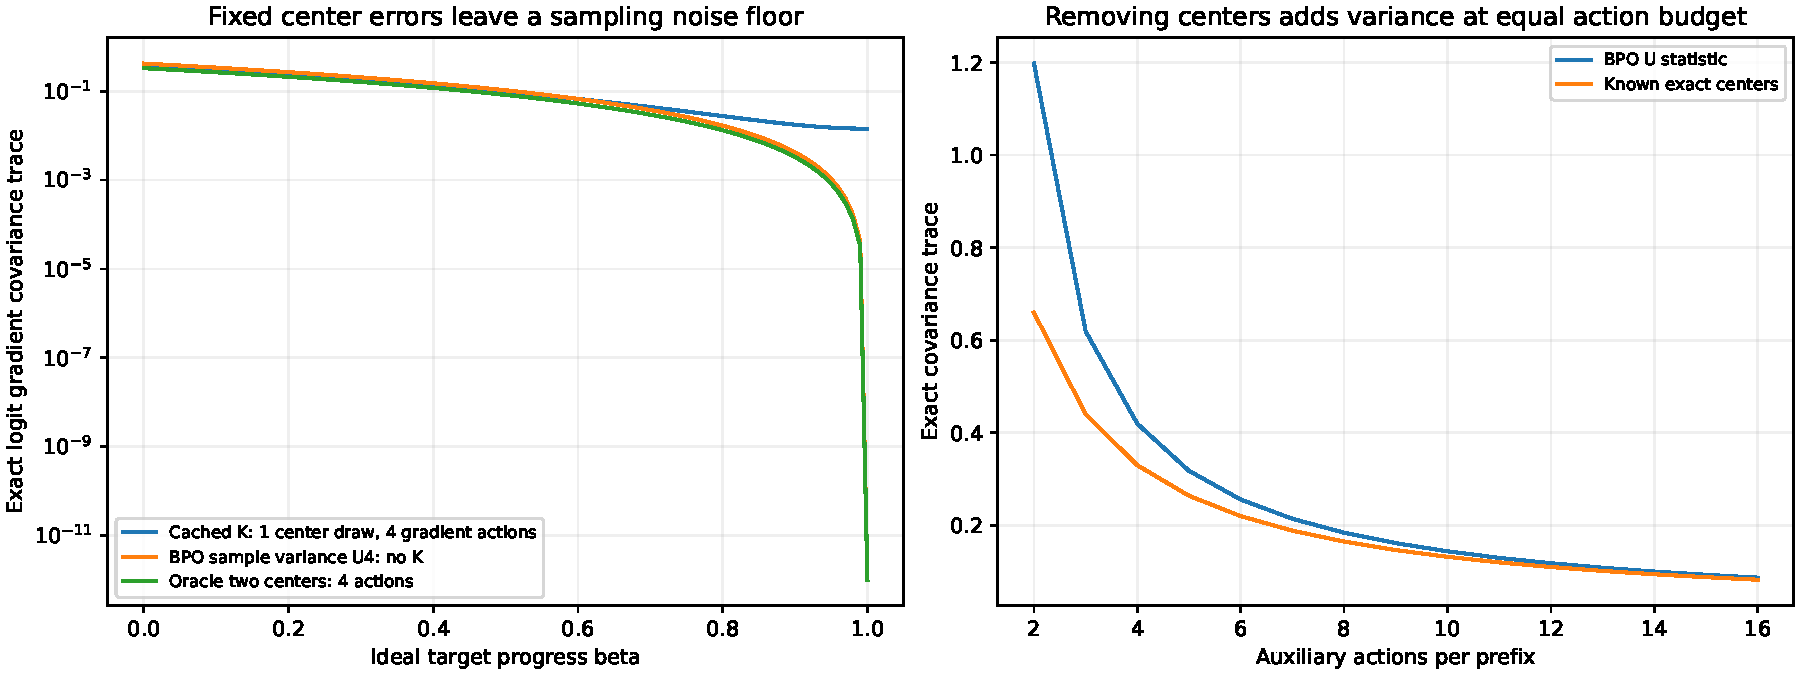
\includegraphics[width=\textwidth]{../../results/power-center-extensions/center-noise-and-sample-variance.pdf}
 \caption{理想 logits 拟合路径上，固定教师中心估计产生末期采样噪声底；BPO sample-variance 梯度的方差随残差平方下降。右图按相同辅助 action 数比较，取消两中心计算有额外方差代价。}
\end{figure}
\begin{figure}[htbp]
 \centering
 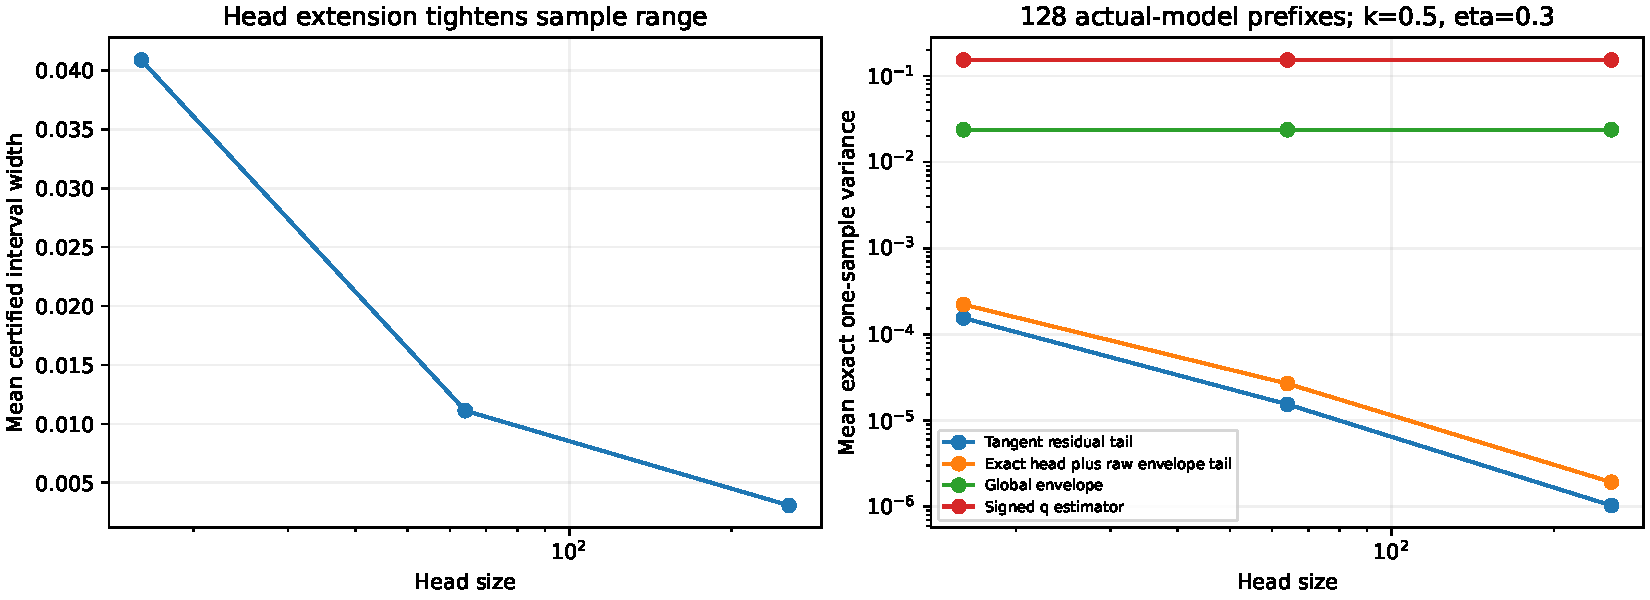
\includegraphics[width=\textwidth]{../../results/power-center-extensions/cached-head-tail-estimation.pdf}
 \caption{原模型缓存 128 个固定前缀上的 tail 区间与无偏估计器条件矩。扩大 head 收紧统一范围与置信保证；实际方差按数据读出，不声称所有输入上都优于其他估计器。}
\end{figure}
